\documentclass[12pt]{article}
% AAU theme adapted from the preamble supplied by the project team.
\usepackage[a4paper,margin=1in]{geometry}
\usepackage{lmodern}
\usepackage[T1]{fontenc}
\usepackage{microtype}
\usepackage{graphicx}
\usepackage{float}
\usepackage{amsmath}
\usepackage[table]{xcolor}
\usepackage{titlesec}
\usepackage{fancyhdr}
\usepackage[most]{tcolorbox}
\PassOptionsToPackage{obeyspaces}{url}
\usepackage[hidelinks]{hyperref}
\usepackage{array}
\usepackage{tabularx}
\usepackage{enumitem}
\usepackage{booktabs}
% Vector UML artwork and multipage test tables.
\usepackage{longtable}
\usepackage{pdflscape}
\definecolor{aauRed}{RGB}{164,22,35}
\definecolor{aauGreen}{RGB}{0,122,88}
\definecolor{darkGray}{RGB}{60,60,60}
\definecolor{softGray}{RGB}{245,245,245}
\pagestyle{fancy}\fancyhf{}\fancyfoot[C]{\thepage}
\renewcommand{\headrulewidth}{0pt}\renewcommand{\footrulewidth}{0pt}
\titleformat{\section}{\normalfont\Large\bfseries\color{aauRed}}{\thesection}{0.6em}{}[{\color{aauRed!65}\titlerule[1.1pt]}]
\titlespacing*{\section}{0pt}{12pt}{8pt}
\titleformat{\subsection}{\normalfont\normalsize\bfseries\color{aauRed!85!black}}{\thesubsection}{0.6em}{}
\titlespacing*{\subsection}{0pt}{10pt}{4pt}
\newtcolorbox{objectivebox}{enhanced,colback=aauRed!5,colframe=aauRed!80!black,boxrule=0.3mm,arc=1mm,left=10pt,right=10pt,top=6pt,bottom=6pt,borderline west={2.5pt}{0pt}{aauRed}}
% Each short use/test case stays on one page, including its heading.
\newtcolorbox{contentbox}[1][]{enhanced,colback=softGray,colframe=black!35,boxrule=0.25mm,arc=2mm,left=9pt,right=9pt,top=7pt,bottom=7pt,before skip=9pt,after skip=9pt,title={\textbf{#1}},fonttitle=\bfseries,coltitle=darkGray,colbacktitle=black!8}
\newcommand{\blankline}{\rule{\linewidth}{0.35pt}}
\newcommand{\insertfigure}[3]{\begin{figure}[H]\centering\fbox{\parbox[c][#2][c]{0.88\textwidth}{\centering\textcolor{black!50}{\Large #1}}}\caption{#3}\end{figure}}
\newcommand{\screen}[3][0.98]{\begin{figure}[H]\centering\includegraphics[width=#1\linewidth]{../assets/#2}\caption{#3}\end{figure}}
% Give wide UML models a dedicated landscape page with readable labels.
\newenvironment{umlpage}{%
\newgeometry{margin=0.65in}\begin{landscape}\pagestyle{empty}%
\AddToHook{shipout/foreground}[arena/umlfooter]{%
\begin{tikzpicture}[remember picture,overlay]
\node[rotate=90,anchor=south,inner sep=0pt] at ([xshift=-23pt]current page.east)
{\normalfont\normalsize\thepage};
\end{tikzpicture}}%
}{\end{landscape}\RemoveFromHook{shipout/foreground}[arena/umlfooter]\pagestyle{fancy}\restoregeometry}
\newcommand{\umlfigure}[2]{\begin{figure}[H]\centering
\includegraphics[width=\linewidth,height=13cm,keepaspectratio]{../assets/uml/#1.pdf}
\caption{#2}\end{figure}}
\providecommand{\reportdate}{10 November 2026}
% Two intentionally sized figures fit together with a heading on an A4 page.
\newcommand{\screenpair}[5][0.30]{%
\begin{figure}[H]\centering
\includegraphics[width=0.96\linewidth,height=#1\textheight,keepaspectratio]{../assets/#2}\caption{#3}
\vspace{8pt}
\includegraphics[width=0.96\linewidth,height=#1\textheight,keepaspectratio]{../assets/#4}\caption{#5}
\end{figure}}
\setlength{\parindent}{0pt}\setlength{\parskip}{5pt}
\setlist[itemize]{leftmargin=1.5em,itemsep=2pt,topsep=3pt}
\setlist[enumerate]{leftmargin=1.7em,itemsep=3pt,topsep=4pt}
\setlength{\emergencystretch}{2em}
\widowpenalty=10000\clubpenalty=10000\displaywidowpenalty=10000
\brokenpenalty=10000
\raggedbottom
\renewcommand{\arraystretch}{1.16}
\setlength{\abovecaptionskip}{7pt}
\setlength{\belowcaptionskip}{4pt}
\setlength{\intextsep}{12pt plus 2pt minus 2pt}
\newcolumntype{Y}{>{\raggedright\arraybackslash}X}
\BeforeBeginEnvironment{tabularx}{\par\noindent}
\AfterEndEnvironment{tabularx}{\par}
\newcommand{\code}[1]{{\small\expandafter\nolinkurl\expandafter{\detokenize{#1}}}}
\newcommand{\command}[1]{\mbox{\small\ttfamily\detokenize{#1}}}
\newcommand{\projecttitle}[2]{%
\hypersetup{pageanchor=false}\begin{titlepage}\centering\vspace*{-0.45cm}
\noindent\begin{minipage}[c]{0.66\textwidth}\raggedright
{\Large\bfseries Al Ain University (AAU)\par}
\end{minipage}\hfill
\begin{minipage}[c]{0.28\textwidth}\raggedleft
% The supplied PNG is unchanged; trim removes only its transparent margins.
\includegraphics[width=3.1cm,trim=1731bp 871bp 1735bp 878bp,clip]{../../aau.png}
\end{minipage}\par
\vspace{0.45cm}
{\scshape\large Object Oriented Analysis and Design\par}
\vspace{0.10cm}
{\normalsize System Analysis \& Design\par}
\vspace{0.10cm}
{\small Course codes: 0103430 \;|\; 0102331\par}
\vspace{0.3cm}\noindent\rule{\linewidth}{0.5mm}\par\vspace{0.3cm}
{\huge\bfseries Arena\par}
\vspace{0.18cm}{\Large\color{aauRed}#1\par}
\vspace{0.15cm}{\normalsize\color{darkGray}#2\par}
\vspace{0.12cm}{\color{aauRed}\rule{\linewidth}{1.2pt}\par}
\vspace{0.35cm}{\normalsize\bfseries Prepared by\par}\vspace{0.15cm}
\begin{tabular}{@{}lr@{}}\textbf{Name}&\textbf{Student ID}\\\midrule
Khaled Alkhawaldeh&202410091\\Abdulrahman Alnaqbi&202340042\\Yousif Alhammadi&202310707\\Ahmed Alsamma&202320192\end{tabular}\par
\vspace{0.22cm}{\color{aauRed!55}\rule{0.6\textwidth}{1.2pt}\par}
\vspace{0.15cm}{\normalsize\textbf{Section:} 61D\par}
\vspace{0.15cm}{\normalsize\textbf{Submitted to:} Dr. Yazeed Ghadi\par}
\vspace{0.3cm}
\begin{tcolorbox}[colback=gray!5,colframe=black!70,title=\textbf{Project Summary},fonttitle=\bfseries,width=0.95\textwidth,boxrule=0.4mm,arc=3mm,left=7pt,right=7pt,top=4pt,bottom=4pt]
A Java desktop workspace for organizing campus competitions, coordinating teams, collecting submissions, evaluating work, and publishing results. Project, programming, and quiz scoring are separated from score-ranking, knockout, and league progression through object-oriented strategies. The application is developed for Al Ain University in the United Arab Emirates.
\end{tcolorbox}
\vfill{\normalsize Fall, 2026--2027\par}{\small Version 2.0 \;|\; \reportdate\par}
\end{titlepage}\pagenumbering{roman}\hypersetup{pageanchor=true}\tableofcontents\clearpage\pagenumbering{arabic}}

\begin{document}
\projecttitle{Interface Mock-ups}{Wireframes, navigation, and implemented screens}
\section{Design Direction}
The Java app and clickable browser prototype share a white navigation rail, burgundy primary actions, warm neutral surfaces, pale green feature panels, serif page headings, and restrained gold accents. A clear page title, a small context label, and a short description establish hierarchy. Tables handle comparison; cards provide entry points without hiding essential rules.

Wireframes are intentionally monochrome. They describe information placement and interaction intent. The screenshot section shows the implemented Swing interface, which adapts the judging wireframe into a submission reader and an evaluation dialog rather than a permanent split pane.
Open \code{prototype/index.html} in a browser for an interactive walkthrough. Its role switch is a demonstration control; the Java app uses authenticated accounts. Both use ten programming problems, a 40/35/25 project rubric, bounded quiz points, and knockout/league match decisions during Active followed by certification and publication. The browser creation form is explicitly a preview; actual creation, account permissions, and persistence are implemented in Java. Their sample events and accounts are independent.

\section{Navigation and Role Paths}
\begin{tabularx}{\linewidth}{lY}\toprule User & Primary path\\\midrule
Student captain & Sign in $\rightarrow$ My teams $\rightarrow$ create team $\rightarrow$ Competition $\rightarrow$ register $\rightarrow$ submit work $\rightarrow$ Results.\\
Student member & Sign in $\rightarrow$ My teams $\rightarrow$ join team before registration $\rightarrow$ view own work and published results.\\
Organizer & Sign in $\rightarrow$ Competitions $\rightarrow$ create draft $\rightarrow$ assign judges $\rightarrow$ open/start/judge/publish.\\
Judge & Sign in $\rightarrow$ Judging studio $\rightarrow$ assigned competition $\rightarrow$ read submission $\rightarrow$ evaluate, or Bracket $\rightarrow$ record winner.\\
Administrator & Sign in $\rightarrow$ People $\rightarrow$ add accounts; Competitions $\rightarrow$ manage any event; Activity $\rightarrow$ review changes.\\\bottomrule\end{tabularx}
\clearpage\section{Low-Fidelity Skeletons}
Editable SVG files are in \code{reports/assets/wireframes}. PNG previews are generated by \code{scripts/generate-wireframes.py}; they are schematic assets, not screenshots.
\screenpair{wireframes/01-overview.png}{Dashboard: featured call to action, metrics, and competition cards.}{wireframes/02-competition.png}{Competition workspace: persistent rules, stage strip, role action, and detail tabs.}
\clearpage
\subsection*{Evaluation and bracket views}
\screenpair{wireframes/03-judging.png}{Judging concept: review context alongside scoring fields. The implementation uses separate reader and scoring dialogs.}{wireframes/04-bracket.png}{Bracket concept: seeded opponents, next-round progression, and champion.}
\clearpage\section{Clickable Browser Prototype}
These captures come from the local HTML/CSS/JavaScript prototype at a 1440-pixel browser viewport. The prototype demonstrates the visual design and interaction flow. It uses a role switch and temporary in-memory sample data; it does not authenticate users or connect to the Java repository. Dates, locations, and event names are illustrative. The Java app implements the service rules and persistence described in the reports.
\screenpair{prototype/01-overview.png}{Browser prototype: overview and discovery cards.}{prototype/02-registration.png}{Browser prototype: project registration workspace.}
\clearpage
\subsection*{Scoring and knockout interactions}
\screenpair{prototype/03-scoring.png}{Browser prototype: live project weighted-score dialog.}{prototype/04-bracket.png}{Browser prototype: active knockout bracket.}
\clearpage\subsection*{Quiz and League Interactions}
\screenpair{prototype/05-quiz.png}{Browser prototype: official quiz points entry for each sample team.}{prototype/06-league.png}{Browser prototype: fixtures and league standings with a draw and completed results.}
\clearpage\subsection*{Creation Preview}
\begin{figure}[H]\centering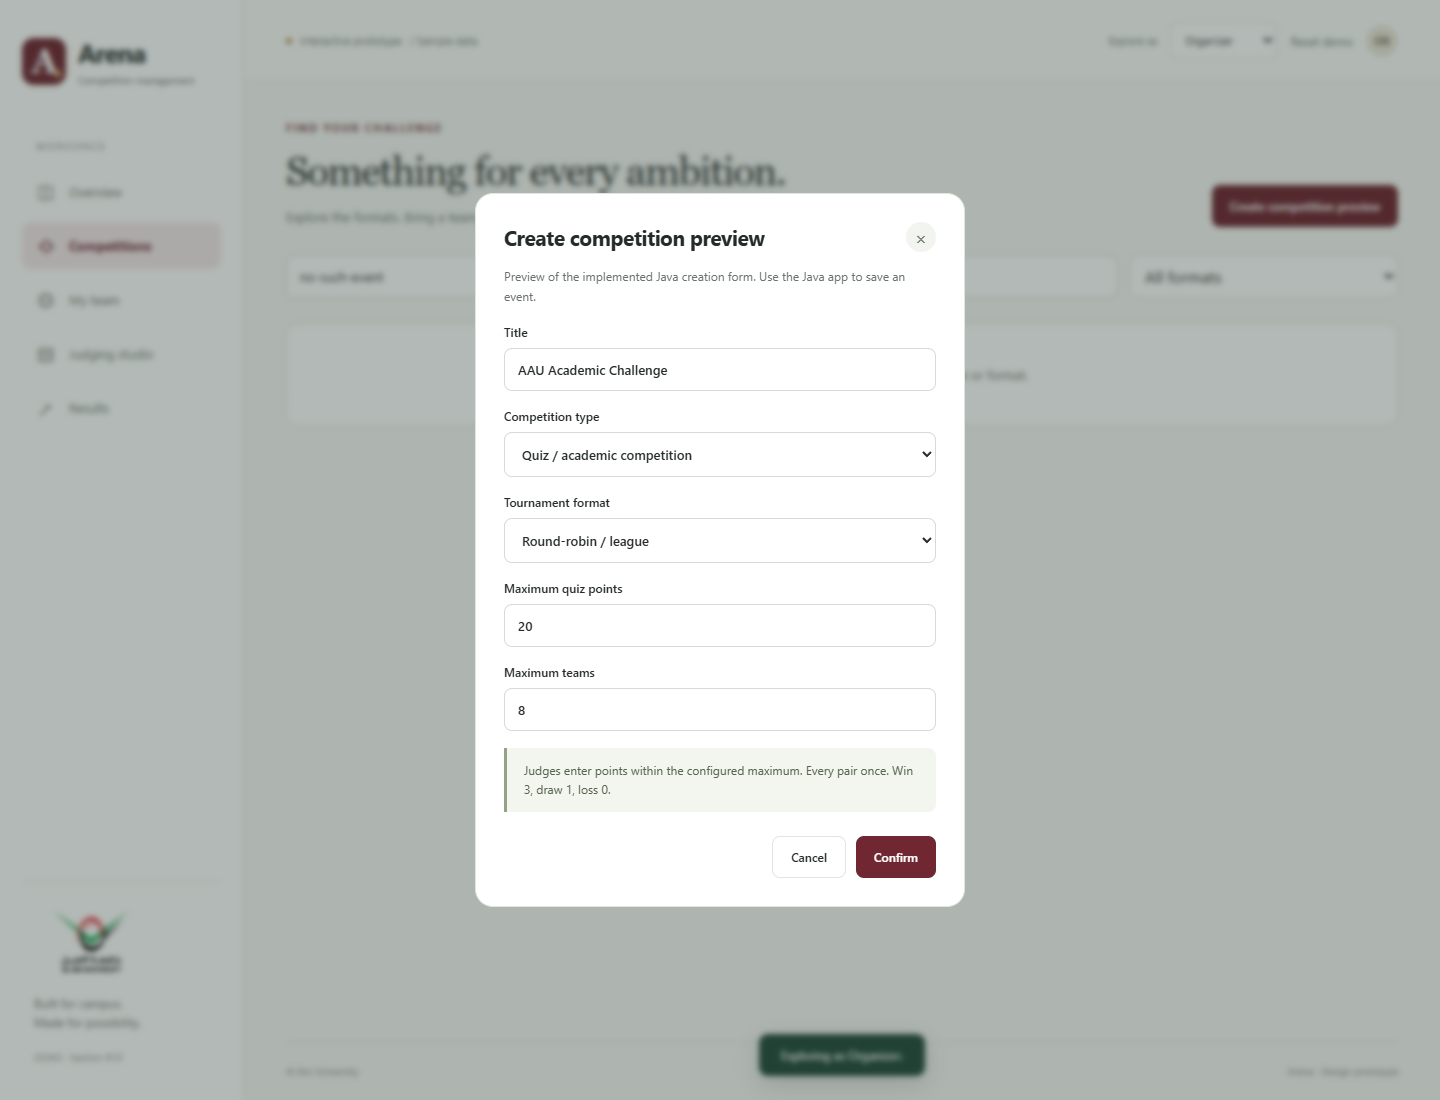
\includegraphics[width=0.90\linewidth,height=0.68\textheight,keepaspectratio]{../assets/prototype/07-creation.png}\caption{Browser creation preview filters formats by competition type. It explicitly directs actual saving to the Java application.}\end{figure}
\clearpage\section{Implemented Screens}
The following images were rendered directly from the actual Swing component tree at a 1440 by 1150 documentation window size using the demonstration dataset. They verify the layout of these screens; they do not constitute a user study or proof that every mouse interaction was manually exercised.
\screenpair{screenshots/01-sign-in.png}{Sign-in screen with a visible local demonstration account.}{screenshots/02-overview.png}{Organizer overview with competition and team metrics.}
\clearpage
\subsection*{Competition discovery and workspace}
\screenpair{screenshots/03-competitions.png}{Competition browsing with text search, format filter, and creation action.}{screenshots/04-competition.png}{Project-format workspace during registration.}
\clearpage
\subsection*{Bracket progression and published results}
\screenpair{screenshots/05-bracket.png}{Active robotics bracket with seeded semifinal matches.}{screenshots/06-results.png}{Published programming leaderboard with score and penalty details.}
\clearpage
\subsection*{Team directory and assigned judging}
\screenpair[0.26]{screenshots/07-teams.png}{Team directory with captain and roster details.}{screenshots/08-judging-studio.png}{Judging studio showing only the current judge's assigned competitions.}
\clearpage\subsection*{League Fixtures and Standings}
\screenpair{screenshots/09-league-fixtures.png}{Actual Swing league fixtures, selected-row scoring action, and publication policy.}{screenshots/12-league-table.png}{Actual manager-only provisional table with played, wins, draws, losses, scores, difference, and points.}
\clearpage\subsection*{Quiz and Match Scoring}
\screenpair{screenshots/11-quiz-score-dialog.png}{Actual quiz scoring dialog with a single relevant points field.}{screenshots/10-match-score-dialog.png}{Actual match-score dialog; league draws are allowed, while knockout draws are rejected.}
\clearpage\subsection*{Competition Creation}
\begin{figure}[H]\centering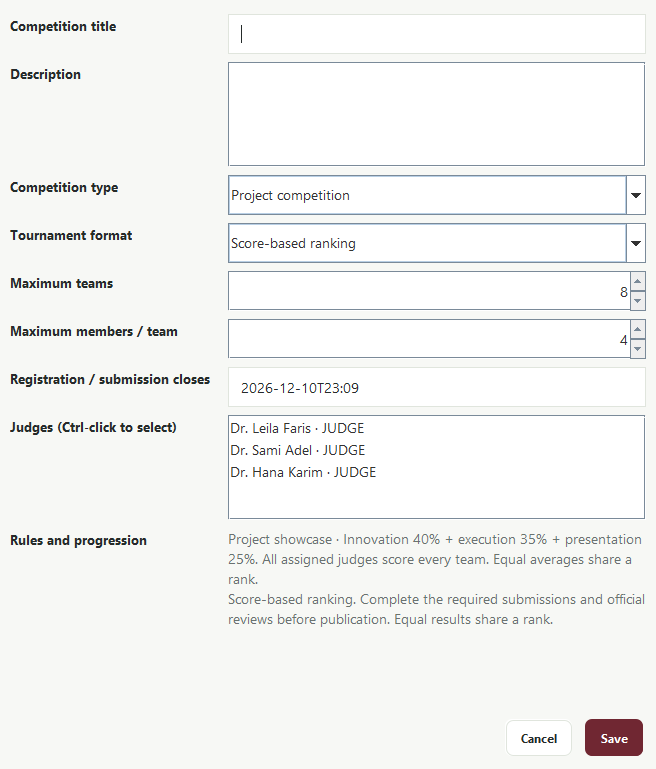
\includegraphics[width=0.90\linewidth,height=0.58\textheight,keepaspectratio]{../assets/screenshots/13-create-competition.png}\caption{Actual creation dialog with separate type and tournament selectors, relevant settings, assigned judges, and rule explanations.}\end{figure}
\section{Interaction States and Accessibility}
Empty result views explain that publication is pending. Missing selections prompt users to choose a row. Invalid input displays a descriptive message without treating the operation as successful. Draft rules become read-only after registration opens. Judges see scoring controls only for assigned events and the appropriate phase.

Controls have descriptive text, Swing keyboard focus, labeled form fields, and table row selection. Textual phase labels supplement color. Long table values have tooltips and submission descriptions can be read in a dedicated dialog. Twenty-two automated Swing checks exercise controls and dialogs, including a live weighted-score preview. Formal screen-reader testing, high-DPI checks, and a usability study remain outstanding.
\end{document}
